%Die Angabe des schlauen Spruchs auf diesem Wege funtioniert nur,
%wenn keine Änderung des Kapitels mittels den in preambel/chapterheads.tex
%vorgeschlagenen Möglichkeiten durchgeführt wurde.
\chapter{Experimental Setup}
\label{chap:chapter5}
%\vspace{-3cm}
%\vspace{2cm}
With the selection of features and their extraction, and the selection of the machine learning algorithm as SVM, explained in earlier chapter, this chapter explains the experimental setup. This chapter focuses on two topics - the first part being the assumptions for the test setup and the configuration of the sample population as well as the method used to generate the sample population, explained in the section~\ref{sec:gsp}. The second part, section~\ref{sec:libsvm}, describes the SVM library used for training and classification of faults and its interface with the generated sample population.
\section{Generation of sample population}
\label{sec:gsp}
The sample population is required to train and cross-validate the machine learning based classifier (hereon referred to simply as \emph{classifier}). A separate set of data is used to test the accuracy of the classifier.
\subsection{Assumptions}
\label{sec:gsp:assumptions}
Following are the assumptions on the sample population and test data:
\begin{enumerate}
  \item It is assumed that the chips to be classified have displayed faulty behavior and hence were rejected in earlier test. For further analysis, the test is run $TestRuns$ times. 
  \item The chips under consideration are either:
		  \begin{enumerate}
    		\item Healthy chips with transient noise or
    		\item Affected by a single permanent or intermittent fault, with or without transient noise.
 		 \end{enumerate}
\end{enumerate}

\subsection{Configuration}
\label{sec:gsp:configuration}
For the purpose of running experiments on different circuits, a sample population and a test set for each of circuit types is created with following configuration:
\begin{enumerate}
  \item A sample population consist of 2500 ($\pm$ 75) of labeled examples. The tolerance of $\pm$ 75 is set as the permanent or intermittent fault instances which did not show any faulty behavior at all at POs, were removed from the sample population.
  \item The sample population is equally divided into following five fault categories:
		\begin{enumerate}
    		\item Permanent faults with the label \texttt{P}.
    		\item Permanent faults along with transient noise (fault rate = 0.001) with the label \texttt{P}.
			\item Intermittent faults (fault rate = 0.1, 0.01 0.001) with the label \texttt{I}.
    		\item Intermittent faults (fault rate = 0.1, 0.01, 0.001) along with transient noise (fault rate = 0.001) with the label \texttt{I}.
			\item Transient faults (fault rate = 0.01, 0.001, 0.0001) with the label \texttt{T}.
 		 \end{enumerate}
	\item Permanent faults are modeled using stuck-at, wired or delay faults, Intermittents are modeled using the high frequency power droop model, and transient faults are modeled as conditional stuck-at faults at random locations, triggered using a deterministic fault rate.
		\item The number of $TestRuns$ to extract features is fixed at 4. This value is set experimentally. 
  \item A test data has 250 ($\pm$ 15) labeled examples, with same configuration as that for the sample population.
\end{enumerate}

The evaluation is done on industrial circuits, kindly provided by NXP. The circuits and the fault coverage test patterns used in the process of generation of sample population is listed in table~\ref{tab:fcov}.
\begin{table}[h]
\captionsetup{justification=centering}
\begin{tabular}{cc}
\hline
\textbf{Circuit} & \textbf{Fault coverage (\%)} \\ \hline
p45k             & 99.56                        \\
p100k            & 99.56                        \\
p141k            & 98.86                        \\
p267k            & 99.60                        \\
p279k            & 97.89                        \\
p295k            & 99.15                       \\
\hline
\end{tabular}
\caption{Fault coverage for circuits used in experiments}
\label{tab:fcov}
\end{table}


\subsection{Implementation}

The sample population is generated as shown in figure~\ref{fig:sampopl} using an in-house simulation framework called Adaptive Diagnosis of Arbitrary Manifold Artifacts (\texttt{ADAMA}). \texttt{ADAMA} can be used for logic simulation with error injection. Logical representation of a circuit at the gate level and a test pattern set are the required inputs for simulation using \texttt{ADAMA}. A fault description can be provided optionally to inject a fault and analyze its behavior. \texttt{ADAMA} supports all of the fault models that have been considered under configuration in section~\ref{sec:gsp:configuration}.




\begin{figure}[h]
  \begin{center}
    \captionsetup{justification=centering}
    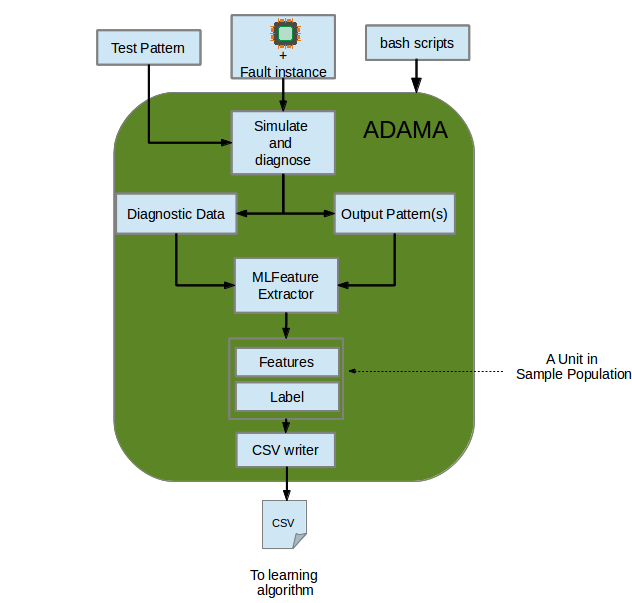
\includegraphics[scale=0.45]{figures/sampopl.png}
    \caption{Generation of sample population using \texttt{ADAMA}}
    \label{fig:sampopl}
  \end{center}
\end{figure}

For the experiments, the \texttt{ADAMA} framework has been extended by adding a task to generate the sample population. The process to generate an example in sample population is illustrated in figure~\ref{fig:sampopl}.

\begin{description}
  \item[Simulation] The simulator is ran $TestRuns$ times after injecting fault instance in the specified circuit description. Output patterns are stored for further analysis. A reference output pattern, without presence of any fault is also generated and stored. 

  \item[Diagnosis] Diagnosis is ran on each set of output patterns corresponding to each simulation run. The diagnostic data generated is stored for a further analysis. 

  \item[Feature extraction] The non-evidence based features are calculated using the reference output and the set of actual output patterns with the extraction process explained in chapter~\ref{chap:chapter4}. The evidence based features are extracted using diagnostic data.

\end{description}

The actual process to generate populations of permanent, transient and intermittent faults is described below:

\begin{description}
  \item[Permanent Faults] \texttt{ADAMA} is used to generate fault descriptions for permanent faults. All fault descriptions are put in a file, and then an instance of \texttt{ADAMA} is invoked to generate examples with permanent faults. Permanent faults with transient noise are generated using same file with fault descriptions, adding a transient fault instance. After generation of features is done, examples which did not result in a failure at POs are check in data for permanent faults. Such examples and their corresponding examples in presence of noise are removed from the sample population.

  \item[Intermittent faults] First intermittent fault descriptions with random seed values for a location and a specified fault activation rate are generated. Then \texttt{ADAMA} is used to simulate these fault instances, first without, and then with a transient noise. The fault descriptions and corresponding examples in feature files of intermittent faults and intermittent faults with transient noise are removed, where intermittent fault as not active, at least for one simulation round.

  \item[Transient faults] The circuit description, along with a transient fault instances, with the specified fault rate are generated and then simulated with \texttt{ADAMA}

\end{description}

\section{Library for SVM based classification - \texttt{LIBSVM}}
\label{sec:libsvm}
\texttt{LIBSVM} \cite{Chang2011} is a popular SVM library, used in a wide variety of applications. It supports linear, polynomial, radial and sigmoid kernel functions and also supports custom user kernels. For experiments, all of the available kernels in the tool have been used, to find out accuracy levels for each of them. It is coded in C++ and Java and it is available as open-source software available for free use under modified BSD license. It supports the multi-class classification using multiple binary classifiers. \texttt{LIBSVM} comes with scripts to train the tool and to find optimal parameters (C and $\gamma$) for classification.

\subsection{Training}

Training module in \texttt{LIBSVM} is basically a QP-solver and it tries to solve the minimization problem described in the section~\ref{mltypes:svm} to find out best fitting model for the  the SVM classifier. To implement a multi-class class classifier, the trainer uses one-vs-one strategy \cite{Knerr1990}. Hence to classify data in $k$-classes, it uses $k(k-1)/2$ classifiers internally \cite{Chang2011}. Each classifier uses two classes for training. The training algorithm algorithm uses $v$-fold cross-validation (CV), meaning that the data is divided into $v$ subsets and one subset $v$ is tested against the classifier trained with rest of the $v-1$ subsets, iteratively until the complete training set is covered \cite{Hsu2003}. This results in the training data being tested once completely. The \emph{cross-validation accuracy} is then calculated as percentage of the data that was correctly classified \cite{Hsu2003}.

\label{sec:impl:tr}
\begin{figure}[h]
  \begin{center}
    \captionsetup{justification=centering}
    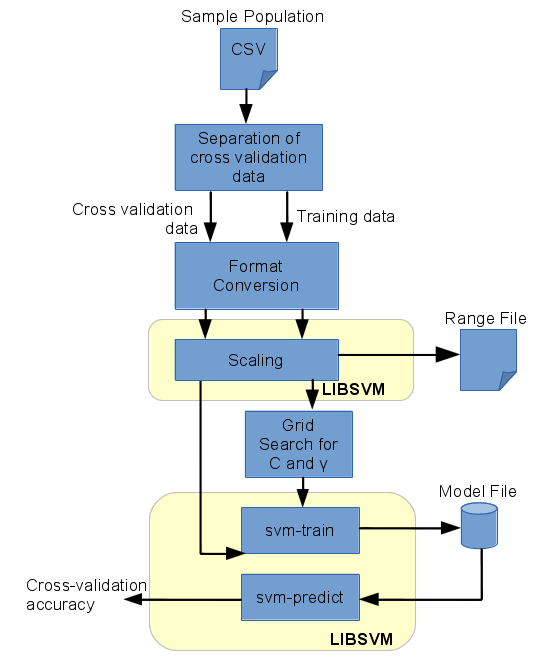
\includegraphics[scale=0.75]{figures/libsvmtrain.png}
    \caption{Steps to train SVM using \texttt{LIBSVM}}
    \label{fig:libsvmtrain}
  \end{center}
\end{figure}

The sequence of steps followed to train SVM, as shown in figure~\ref{fig:libsvmtrain} is as follows:
\begin{description}

  \item[Scaling] The scaling module in \texttt{LIBSVM} provides functionality to scale the training data to user specified input range. The documentation of \texttt{LIBSVM} \cite{Hsu2003} suggest the use of range [0,1] for the data containing zero values for some of features, as in our case. The scaling parameters are stored in a \emph{range file}, which is later used to scale features of future examples or the test data.

   \item[Training] Trainer executable file in \texttt{LIBSVM} is used for training the SVM. The training data and the kernel to be used for training needs to be provided as an input at this stage. It outputs a \emph{model file} to be used for prediction of future examples.

  \item[Grid search for $C$ and $\gamma$] \texttt{LIBSVM} provides a script to find suitable values of C and $\gamma$. The grid search  algorithm tries various pairs of C and $\gamma$ to find a pair with the highest CV accuracy, heuristically. This script internally uses the training module for modeling classifiers, hence the kernel type for training needs to be specified. A common value of $C$ and $\gamma$ is searched and applied to all internal classifiers. The \emph{class-weights} can be then applied, which is a simple multiplier to the parameter $C$ of that particular class, to fine-tune the classifier \cite{Chang2011}.
 
\end{description}

\subsection{Classification}

In the classification of the multi-class data, the classifier uses a voting strategy. Each of the classifiers votes for a given input example. The example is assigned a class with the maximum number of votes. In case that two classes have identical votes, classifier simply choose the class appearing first in the array of storing class names \cite{Chang2011}. However this is not possible in our case as we use 3 classes, and hence, 3 binary classifiers internally.

Steps to classify data using already trained SVM is shown in figure~\ref{fig:libsvmpredict}. A short description of the these is noted below:

\begin{figure}[h]
  \begin{center}
    \captionsetup{justification=centering}
    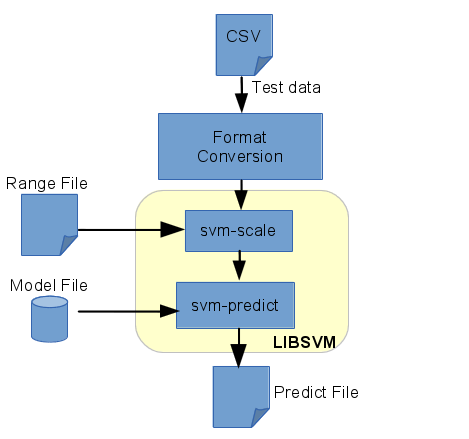
\includegraphics[scale=0.75]{figures/libsvmpredict.png}
    \caption{Steps for classification of test data with SVM using \texttt{LIBSVM}}
    \label{fig:libsvmpredict}
  \end{center}
\end{figure}

\begin{description}

  \item[Scaling] The test data is scaled using same scaling module used for training. The range file generated while scaling the training data is used in this step to scale the test data, instead of manually specifying ranges.
  
  \item[Prediction] The prediction tool provided with \texttt{LIBSVM} is used to predict the test data. This tool needs model file generated during training as an input and it then outputs a \emph{predict file} with predicated labels of the test data. This file is further processed using scripts for the evaluation of accuracy levels of different fault classes.
  
\end{description}
